\subsection{UC6: Gestione dashboard}
\hypertarget{UC6}{}
\begin{figure} [H]
	\centering
	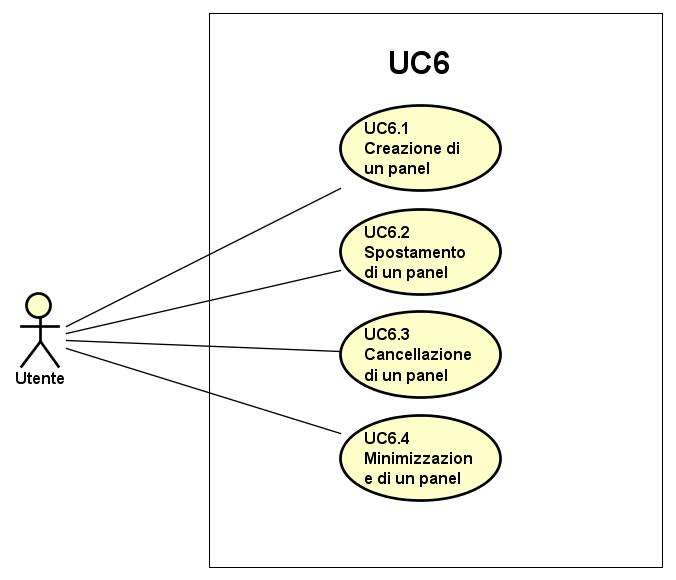
\includegraphics[scale=0.45]{Img/UC6}
	\caption{UC6: Gestione dashboard}\label{}
\end{figure}
\begin{itemize}
	\item \textbf{Attori}: Utente;
	\item \textbf{Scopo e descrizione}: L'attore configura la disposizione dei \gl{panel} nella \gl{dashboard};
	\item \textbf{Precondizione}: La rete Bayesiana deve essere configurata;
	\item \textbf{Flusso principale degli eventi}:
	\begin{itemize}
		\item Creazione di un panel  (UC6.1);
		\item Spostamento di un panel  (UC6.2);
		\item Cancellazione di un panel  (UC6.3);
		\item \gl{Minimizzazione} di un panel  (UC6.4).
	\end{itemize}
	\item \textbf{Postcondizione}: La dashboard contiene i panel voluti dall'utente seguendo le sue disposizioni.
\end{itemize}
\subsection{UC6.1: Creazione di un panel}
\hypertarget{UC6.1}{}
\begin{itemize}
	\item \textbf{Attori}: Utente;
	\item \textbf{Scopo e descrizione}: L'utente crea un panel a scelta tra Graph, Singlestat Panel, Dashboard List Panel, Table Panel, Text Panel e ne configura i valori;
	\item \textbf{Precondizione}: Il sistema permette la creazione di un nuovo panel;
	\item \textbf{Flusso principale degli eventi}:
	\begin{itemize}
		\item L'utente seleziona la funzionalità "Crea panel";
		\item L'utente seleziona una tipologia di panel tra quelli a scelta;
		\item L'utente configura il panel (UC7.1).
	\end{itemize}
	\item \textbf{Postcondizione}: Il panel è stato creato e configurato.
\end{itemize}
\subsection{UC6.2: Spostamento di un panel}
\hypertarget{UC6.2}{}
\begin{itemize}
	\item \textbf{Attori}: Utente;
	\item \textbf{Scopo e descrizione}: L'utente può spostare il panel dentro la dashboard;
	\item \textbf{Precondizione}: La dashboard è stata caricata e l'utente vuole spostare il panel;
	\item \textbf{Postcondizione}: La dashboard ha subito lo spostamento del panel come desiderato dall'utente.
\end{itemize}
\subsection{UC6.3: Cancellazione di un panel}
\hypertarget{UC6.3}{}
\begin{itemize}
	\item \textbf{Attori}: Utente;
	\item \textbf{Scopo e descrizione}: L'utente può cancellare il panel dentro la dashboard;
	\item \textbf{Precondizione}: La dashboard è stata caricata e l'utente vuole cancellare il panel;
	\item \textbf{Postcondizione}: La dashboard ha subito la cancellazione del panel come desiderato dall'utente.
\end{itemize}
\subsection{UC6.4: Minimizzazione di un panel}
\hypertarget{UC6.4}{}
\begin{itemize}
	\item \textbf{Attori}: Utente;
	\item \textbf{Scopo e descrizione}: L'utente può minimizzazione il panel dentro la dashboard;
	\item \textbf{Precondizione}: La dashboard è stata caricata e l'utente vuole minimizzazione il panel;
	\item \textbf{Postcondizione}: La dashboard ha subito la minimizzazione del panel come desiderato dall'utente.
\end{itemize}
\subsection{UC7: Visualizzazione dati tramite dashboard}
\hypertarget{UC7}{}
\begin{figure} [H]
	\centering
	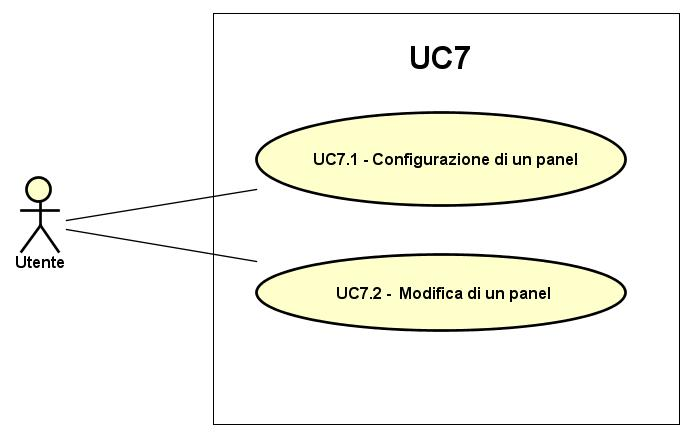
\includegraphics[scale=0.45]{Img/UC7}
	\caption{UC7: Visualizzazione dati tramite dashboard}\label{}
\end{figure}
\begin{itemize}
	\item \textbf{Attori}: Utente;
	\item \textbf{Scopo e descrizione}: L'attore configura e/o modifica le opzioni relative alla visualizzazione dei dati nei panel;
	\item \textbf{Precondizione}: La dashboard e i panel sono stati caricati;
	\item \textbf{Flusso principale degli eventi}:
	\begin{itemize}
		\item Configurazione di un panel (UC7.1);
		\item Modifica di un panel (UC7.2).
	\end{itemize}
	\item \textbf{Postcondizione}: I panel sono stati configurati e/o modificati.
\end{itemize}
\subsection{UC7.1: Configurazione di un panel}
\hypertarget{UC7.1}{}
\begin{figure} [H]
	\centering
	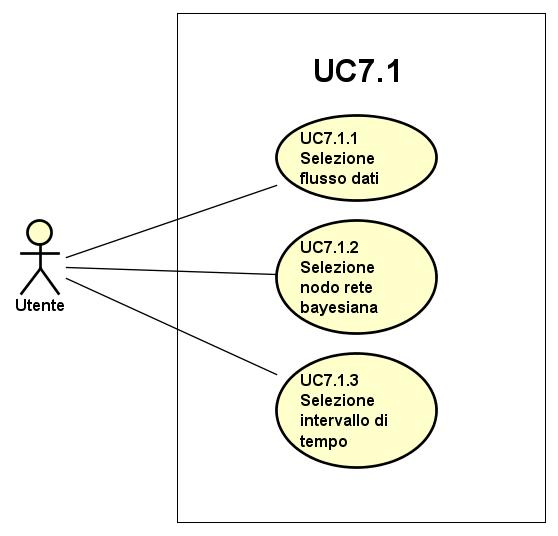
\includegraphics[scale=0.45]{Img/UC7-1}
	\caption{UC7.1: Configurazione di un panel}\label{}
\end{figure}
\begin{itemize}
	\item \textbf{Attori}: Utente;
	\item \textbf{Scopo e descrizione}: L'attore configura le opzioni relative alla visualizzazione dei dati nei panel;
	\item \textbf{Precondizione}: La dashboard e il panel che si vuole configurare sono stati caricati;
	\item \textbf{Flusso principale degli eventi}:
	\begin{itemize}
		\item Selezione flusso dati  (UC7.1.1);
		\item Selezione nodo rete Bayesiana(UC7.1.2);
		\item Selezione intervallo di tempo (UC7.1.3).		
	\end{itemize}
	\item \textbf{Postcondizione}: Il panel è stato configurato.
\end{itemize}
\subsection{UC7.1.1: Selezione flusso dati}
\hypertarget{UC7.1.1}{}
\begin{itemize}
	\item \textbf{Attori}: Utente;
	\item \textbf{Scopo e descrizione}: L'utente può selezionare il flusso di dati dentro il panel;
	\item \textbf{Precondizione}: La dashboard e il panel che si vuole configurare sono stati caricati e l'utente vuole selezionare il flusso di dati dentro il panel;
	\item \textbf{Postcondizione}: Il panel ha subito la selezione del flusso di dati scelto dall'utente.
\end{itemize}
\subsection{UC7.1.2: Selezione nodo rete Bayesiana }
\hypertarget{UC7.1.2}{}
\begin{itemize}
	\item \textbf{Attori}: Utente;
	\item \textbf{Scopo e descrizione}: L'utente può selezionare il nodo della rete Bayesiana da visualizzare dentro il panel;
	\item \textbf{Precondizione}: La dashboard e il panel che si vuole configurare sono stati caricati e l'utente vuole selezionare il nodo della rete Bayesiana da visualizzare dentro il panel;
	\item \textbf{Postcondizione}: Il panel ha subito la selezione del nodo scelto dall'utente.
\end{itemize}
\subsection{UC7.1.3: Selezione intervallo di tempo  }
\hypertarget{UC7.1.3}{}
\begin{itemize}
	\item \textbf{Attori}: Utente;
	\item \textbf{Scopo e descrizione}: L'utente può selezionare l'intervallo di tempo da visualizzare dentro il panel;
	\item \textbf{Precondizione}: La dashboard e il panel che si vuole configurare sono stati caricati e l'utente vuole selezionare l'intervallo di tempo da visualizzare dentro il panel;
	\item \textbf{Postcondizione}: Il panel ha subito la selezione dell'intervallo di tempo scelto dall'utente.
\end{itemize}
\subsection{UC7.2: Modifica di un panel}
\hypertarget{UC7.2}{}
\begin{figure} [H]
	\centering
	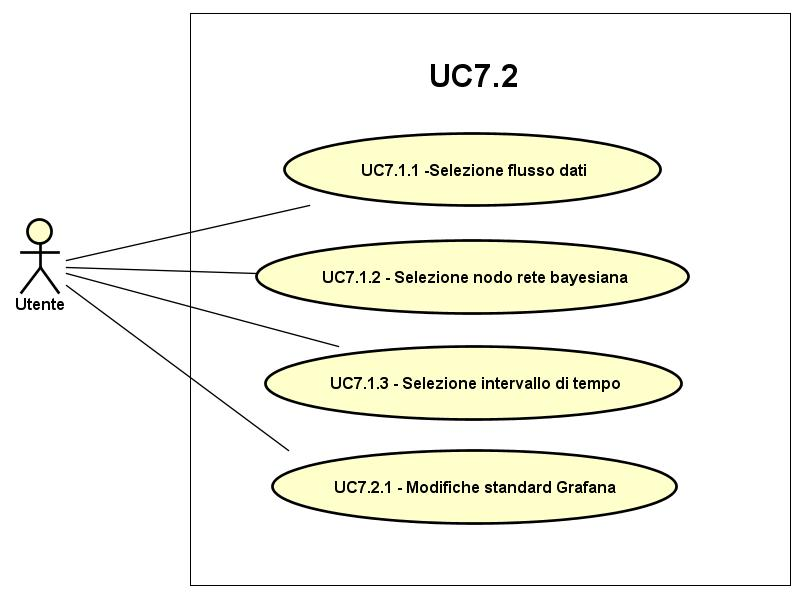
\includegraphics[scale=0.45]{Img/UC7-2}
	\caption{UC7.1: Modifica di un panel}\label{}
\end{figure}
\begin{itemize}
	\item \textbf{Attori}: Utente;
	\item \textbf{Scopo e descrizione}: L'attore modifica le opzioni relative alla visualizzazione dei dati nei panel;
	\item \textbf{Precondizione}: La dashboard e il panel che si vuole modificare sono stati caricati;
	\item \textbf{Flusso principale degli eventi}:
	\begin{itemize}
		\item Selezione flusso dati  (UC7.1.1);
		\item Selezione nodo rete Bayesiana(UC7.1.2);
		\item Selezione intervallo di tempo (UC7.1.3);
		\item Modifiche standard Grafana  (UC7.2.1).		
	\end{itemize}
	\item \textbf{Postcondizione}: Il panel è stato modificato.
\end{itemize}
\subsection{UC7.2.1: Modifiche standard Grafana}
\hypertarget{UC7.2.1}{}
\begin{itemize}
	\item \textbf{Attori}: Utente;
	\item \textbf{Scopo e descrizione}: L'utente può effettuare le modifiche standard previste da Grafana dentro il panel;
	\item \textbf{Precondizione}: La dashboard e il panel che si vuole modificare sono stati caricati e l'utente vuole effettuare le modifiche standard previste da Grafana dentro il panel;
	\item \textbf{Postcondizione}: Il panel ha subito le modifiche standard previste da Grafana scelto dall'utente.
\end{itemize}